\SourcePage{438}{441}
\section{Point groups}

For the transformations in the symmetry group of a finite body (a molecule in particular), there must be at least one point of the body that every transformation leaves fixed. Equivalently, all its symmetry axes and planes must share at least one point. Indeed, successive rotations about two nonintersecting axes, or reflections in nonintersecting planes, produce a translation of the body; such a displacement plainly cannot bring a finite body into coincidence with itself. Symmetry groups having this property are called \emph{point groups}.

Before constructing the possible kinds of point groups, consider a simple geometric device for assigning their elements to classes. Let $Oa$ be an axis, and let the group element $A$ rotate through a certain angle about it. Suppose another transformation $G$ of the same group, whether a rotation or a reflection, carries the axis $Oa$ itself into the position $Ob$. We claim that $B=GAG^{-1}$ is then a rotation about $Ob$ through the same angle as $A$ about $Oa$. To see this, apply $GAG^{-1}$ to the axis $Ob$. First $G^{-1}$ takes $Ob$ to $Oa$; the ensuing rotation $A$ leaves that axis in place; and $G$ finally returns it to its original position. Thus $Ob$ remains fixed, so $B$ is a rotation about that axis. Moreover, $A$ and $B$ lie in one class and consequently have the same order, which means that their rotation angles are equal.

It follows that two rotations through an equal angle belong to the same class whenever the group contains a transformation superposing one rotation axis on the other. The same reasoning shows that reflections in two different planes are in one class if some group transformation takes one plane into the other. Symmetry

\SourcePage{439}{442}
axes or planes whose directions can be superposed in this way are termed \emph{equivalent}.

When both rotations are about the same axis, a few further observations are needed. The inverse of $C_n^k$ ($k=1,2,\ldots,n-1$), a rotation about an $n$-fold symmetry axis, is $C_n^{-k}=C_n^{n-k}$. It is a rotation through $(n-k)(2\pi/n)$ in the original sense, or equivalently through $2k\pi/n$ in the opposite sense. If the group includes a rotation through $\pi$ about a perpendicular axis, which reverses the direction of the axis under consideration, then the general result just proved places $C_n^k$ and $C_n^{-k}$ in the same class. Reflection $\sigma_h$ in a plane perpendicular to the axis also reverses its direction, but a reflection reverses the sense of rotation as well. Hence the presence of $\sigma_h$ does not make $C_n^k$ and $C_n^{-k}$ conjugate. By contrast, reflection $\sigma_v$ in a plane containing the axis preserves the direction of that axis while reversing the sense of rotation. Thus $C_n^{-k}=\sigma_vC_n^k\sigma_v$, and such a symmetry plane makes $C_n^k$ and $C_n^{-k}$ members of one class. An axis for which equal rotations in opposite senses are conjugate will be called \emph{two-sided}.

The following rule often simplifies the determination of the classes of a point group. Let $\boldsymbol{G}$ be a group without the inversion $I$, and let $\boldsymbol{C}_i$ consist of the two elements $I$ and $E$. The direct product $\boldsymbol{G}\times\boldsymbol{C}_i$ has twice as many elements as $\boldsymbol{G}$: one half are the elements of $\boldsymbol{G}$ themselves, and the other half are obtained by multiplying them by $I$. Since $I$ commutes with every point-group transformation, $\boldsymbol{G}\times\boldsymbol{C}_i$ likewise has twice the number of classes of $\boldsymbol{G}$. Each class $A$ of $\boldsymbol{G}$ gives the two classes $A$ and $AI$ in the product group. In particular, inversion $I$ always forms a class by itself.

We now list all possible point groups, beginning with the simplest and adjoining new symmetry elements in succession. Point groups will be denoted by bold Latin letters with suitable subscripts.

\medskip
\noindent I. Group $\boldsymbol{C}_n$

The simplest symmetry type has only one $n$-fold symmetry axis. The group $\boldsymbol{C}_n$ consists of rotations about this axis and is plainly cyclic. Each of its $n$ elements is a separate class. The group $\boldsymbol{C}_1$

\SourcePage{440}{443}
contains only the identity transformation $E$ and thus corresponds to complete absence of symmetry.

\medskip
\noindent II. Group $\boldsymbol{S}_{2n}$

This is the group generated by a rotation--reflection axis of even order $2n$. It has $2n$ elements and is cyclic. In particular, $\boldsymbol{S}_2$ has only the elements $E$ and $I$ and is also written $\boldsymbol{C}_i$. Notice also that when the group order has the form $2n=4p+2$, inversion is one of its elements, since $(S_{4p+2})^{2p+1}=C_2\sigma_h=I$. Such a group can be expressed as the direct product $\boldsymbol{S}_{4p+2}=\boldsymbol{C}_{2p+1}\times\boldsymbol{C}_i$ and is also denoted by $\boldsymbol{C}_{2p+1,i}$.

\medskip
\noindent III. Group $\boldsymbol{C}_{nh}$

This group results when a symmetry plane perpendicular to an $n$-fold symmetry axis is adjoined. The $2n$ elements of $\boldsymbol{C}_{nh}$ are the $n$ rotations of $\boldsymbol{C}_n$ and the $n$ rotation--reflection transformations $C_n^k\sigma_h$ ($k=1,2,3,\ldots,n$), including the reflection $C_n^n\sigma_h=\sigma_h$. Every pair of elements commutes, so the group is Abelian and has as many classes as elements. For even $n$ ($n=2p$) it contains a center of symmetry, because $C_{2p}^p\sigma_h=C_2\sigma_h=I$. The simplest group $\boldsymbol{C}_{1h}$ has just $E$ and $\sigma_h$ and is also called $\boldsymbol{C}_s$.

\medskip
\noindent IV. Group $\boldsymbol{C}_{nv}$

Adjoining to an $n$-fold symmetry axis a symmetry plane that contains it automatically supplies another $(n-1)$ planes, all intersecting along the axis at angles $\pi/n$. This follows immediately from the geometrical theorem (91.7).\footnote{A finite group cannot contain two symmetry planes meeting at an angle that is not a rational fraction of $2\pi$. Two such planes would imply infinitely many further symmetry planes through the same line, generated by reflecting either plane in the other without limit. In other words, two planes of this kind at once imply full axial symmetry.} The resulting group $\boldsymbol{C}_{nv}$ therefore has $2n$ elements: $n$ rotations about the $n$-fold axis and $n$ reflections $\sigma_v$ in vertical planes. Figure~34 shows, as examples, the axes and symmetry planes of $\boldsymbol{C}_{3v}$ and $\boldsymbol{C}_{4v}$.

In finding the classes, first note that the symmetry planes containing the axis make this axis

\SourcePage{441}{444}
two-sided. The actual division of the elements into classes differs for even and odd $n$.

\begin{figure}[ht]
\centering
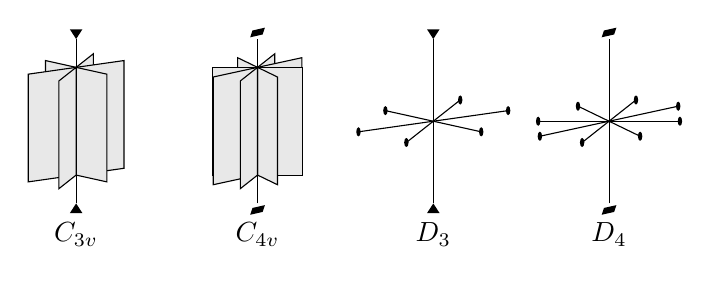
\begin{tikzpicture}[scale=.72,line width=.4pt]
\draw[fill=gray!18] (0,-0.95)--(0.304,-0.71)--(0.304,1.19)--(0,0.95)--cycle;
\draw[fill=gray!18] (0,-0.95)--(0.845,-0.83)--(0.845,1.07)--(0,0.95)--cycle;
\draw[fill=gray!18] (0,-0.95)--(-0.541,-0.83)--(-0.541,1.07)--(0,0.95)--cycle;
\draw[fill=gray!18] (0,-0.95)--(-0.845,-1.07)--(-0.845,0.83)--(0,0.95)--cycle;
\draw[fill=gray!18] (0,-0.95)--(0.541,-1.07)--(0.541,0.83)--(0,0.95)--cycle;
\draw[fill=gray!18] (0,-0.95)--(-0.304,-1.19)--(-0.304,0.71)--(0,0.95)--cycle;
\draw (0,-1.45)--(0,1.45);\fill (0,1.45)--(-0.11,1.6199999999999999)--(0.11,1.6199999999999999)--cycle;\fill (0,-1.45)--(-0.11,-1.6199999999999999)--(0.11,-1.6199999999999999)--cycle;\node at (0,-2.0) {$C_{3v}$};
\draw[fill=gray!18] (3.2,-0.95)--(3.504,-0.71)--(3.504,1.19)--(3.2,0.95)--cycle;
\draw[fill=gray!18] (3.2,-0.95)--(2.849,-0.78)--(2.849,1.12)--(3.2,0.95)--cycle;
\draw[fill=gray!18] (3.2,-0.95)--(3.981,-0.78)--(3.981,1.12)--(3.2,0.95)--cycle;
\draw[fill=gray!18] (3.2,-0.95)--(4,-0.95)--(4,0.95)--(3.2,0.95)--cycle;
\draw[fill=gray!18] (3.2,-0.95)--(2.4,-0.95)--(2.4,0.95)--(3.2,0.95)--cycle;
\draw[fill=gray!18] (3.2,-0.95)--(2.419,-1.12)--(2.419,0.78)--(3.2,0.95)--cycle;
\draw[fill=gray!18] (3.2,-0.95)--(3.551,-1.12)--(3.551,0.78)--(3.2,0.95)--cycle;
\draw[fill=gray!18] (3.2,-0.95)--(2.896,-1.19)--(2.896,0.71)--(3.2,0.95)--cycle;
\draw (3.2,-1.45)--(3.2,1.45);\fill (3.0700000000000003,1.48)--(3.29,1.53)--(3.33,1.65)--(3.1100000000000003,1.5999999999999999)--cycle;\fill (3.0700000000000003,-1.65)--(3.29,-1.5999999999999999)--(3.33,-1.48)--(3.1100000000000003,-1.53)--cycle;\node at (3.2,-2.0) {$C_{4v}$};
\draw (6.3,-1.45)--(6.3,1.45);\fill (6.3,1.45)--(6.1899999999999995,1.6199999999999999)--(6.41,1.6199999999999999)--cycle;\fill (6.3,-1.45)--(6.1899999999999995,-1.6199999999999999)--(6.41,-1.6199999999999999)--cycle;\draw (4.98,-0.187)--(7.62,0.187);\fill (4.98,-0.187) ellipse[x radius=1.1pt,y radius=2.3pt];\fill (7.62,0.187) ellipse[x radius=1.1pt,y radius=2.3pt];\draw (5.825,-0.375)--(6.775,0.375);\fill (5.825,-0.375) ellipse[x radius=1.1pt,y radius=2.3pt];\fill (6.775,0.375) ellipse[x radius=1.1pt,y radius=2.3pt];\draw (7.145,-0.187)--(5.455,0.187);\fill (7.145,-0.187) ellipse[x radius=1.1pt,y radius=2.3pt];\fill (5.455,0.187) ellipse[x radius=1.1pt,y radius=2.3pt];\node at (6.3,-2.0) {$D_3$};
\draw (9.4,-1.45)--(9.4,1.45);\fill (9.27,1.48)--(9.49,1.53)--(9.530000000000001,1.65)--(9.31,1.5999999999999999)--cycle;\fill (9.27,-1.65)--(9.49,-1.5999999999999999)--(9.530000000000001,-1.48)--(9.31,-1.53)--cycle;\draw (8.15,-0)--(10.65,0);\fill (8.15,-0) ellipse[x radius=1.1pt,y radius=2.3pt];\fill (10.65,0) ellipse[x radius=1.1pt,y radius=2.3pt];\draw (8.18,-0.265)--(10.62,0.265);\fill (8.18,-0.265) ellipse[x radius=1.1pt,y radius=2.3pt];\fill (10.62,0.265) ellipse[x radius=1.1pt,y radius=2.3pt];\draw (8.925,-0.375)--(9.875,0.375);\fill (8.925,-0.375) ellipse[x radius=1.1pt,y radius=2.3pt];\fill (9.875,0.375) ellipse[x radius=1.1pt,y radius=2.3pt];\draw (9.948,-0.265)--(8.852,0.265);\fill (9.948,-0.265) ellipse[x radius=1.1pt,y radius=2.3pt];\fill (8.852,0.265) ellipse[x radius=1.1pt,y radius=2.3pt];\node at (9.4,-2.0) {$D_4$};
\end{tikzpicture}
\caption{}
\label{fig:93-34}
\end{figure}

For odd $n$ ($n=2p+1$), successive rotations $C_{2p+1}$ carry any one plane into each of the other $2p$ planes. All the symmetry planes are therefore equivalent, and their reflections belong to a single class. Among the axial rotations there are $2p$ nonidentity operations; conjugate pairs form $p$ two-element classes ($C_{2p+1}^k$ and $C_{2p+1}^{-k}$, $k=1,2,\ldots,p$). The identity $E$ supplies one further class, giving $p+2$ classes altogether.

For even $n$ ($n=2p$), successive rotations $C_{2p}$ superpose only alternate planes; adjacent planes cannot be brought into coincidence. There are consequently two sets of $p$ equivalent planes, and hence two classes containing $p$ reflections each. Of the axial rotations, $C_{2p}^{2p}=E$ and $C_{2p}^p=C_2$ each form a class alone. The remaining $2p-2$ rotations occur in conjugate pairs, producing another $p-1$ two-element classes. Thus $\boldsymbol{C}_{2p,v}$ has $p+3$ classes in all.

\medskip
\noindent V. Group $\boldsymbol{D}_n$

When a twofold axis perpendicular to an $n$-fold symmetry axis is adjoined, another $(n-1)$ such axes appear. There are then $n$ horizontal twofold axes meeting at angles $\pi/n$. The resulting group $\boldsymbol{D}_n$ has $2n$ elements: $n$ rotations about the $n$-fold axis and $n$ rotations through $\pi$ about the horizontal axes. We shall denote the latter by $U_2$, reserving $C_2$ for rotation through $\pi$ about the vertical

\SourcePage{442}{445}
axis. Figure~34 also shows the axial systems of $\boldsymbol{D}_3$ and $\boldsymbol{D}_4$ as examples.

Exactly as in the preceding case, the $n$-fold axis is two-sided. For odd $n$ all the horizontal twofold axes are equivalent, whereas for even $n$ they split into two inequivalent sets. The $p+3$ classes of $\boldsymbol{D}_{2p}$ are therefore $E$, two classes each containing $p$ rotations $U_2$, the rotation $C_2$, and $(p-1)$ classes each containing two rotations about the vertical axis. The group $\boldsymbol{D}_{2p+1}$ instead has $p+2$ classes: $E$, one class of $2p+1$ rotations $U_2$, and $p$ two-element classes of rotations about the vertical axis.

An important special case is $\boldsymbol{D}_2$, whose axial system consists of three mutually perpendicular twofold axes. This group is also denoted by $\boldsymbol{V}$.

\medskip
\noindent VI. Group $\boldsymbol{D}_{nh}$

Add to the axes of $\boldsymbol{D}_n$ a horizontal symmetry plane containing its $n$ twofold axes. This automatically creates $n$ vertical planes, each containing the vertical axis and one horizontal axis. The resulting group $\boldsymbol{D}_{nh}$ has $4n$ elements. Besides the $2n$ elements of $\boldsymbol{D}_n$, it includes $n$ reflections $\sigma_v$ and $n$ rotation--reflection transformations $C_n^k\sigma_h$. The axes and planes of $\boldsymbol{D}_{3h}$ are shown in Fig.~35.

\begin{figure}[ht]
\centering
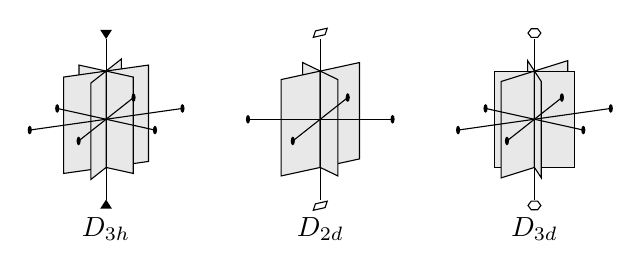
\begin{tikzpicture}[scale=.68,line width=.4pt]
\draw[fill=gray!18] (0,-0.9)--(0.285,-0.675)--(0.285,1.125)--(0,0.9)--cycle;
\draw[fill=gray!18] (0,-0.9)--(0.792,-0.788)--(0.792,1.012)--(0,0.9)--cycle;
\draw[fill=gray!18] (0,-0.9)--(-0.507,-0.788)--(-0.507,1.012)--(0,0.9)--cycle;
\draw[fill=gray!18] (0,-0.9)--(-0.792,-1.012)--(-0.792,0.788)--(0,0.9)--cycle;
\draw[fill=gray!18] (0,-0.9)--(0.507,-1.012)--(0.507,0.788)--(0,0.9)--cycle;
\draw[fill=gray!18] (0,-0.9)--(-0.285,-1.125)--(-0.285,0.675)--(0,0.9)--cycle;
\draw (-1.426,-0.202)--(1.426,0.202);\fill (-1.426,-0.202) ellipse[x radius=1.1pt,y radius=2.3pt];\fill (1.426,0.202) ellipse[x radius=1.1pt,y radius=2.3pt];\draw (-0.513,-0.405)--(0.513,0.405);\fill (-0.513,-0.405) ellipse[x radius=1.1pt,y radius=2.3pt];\fill (0.513,0.405) ellipse[x radius=1.1pt,y radius=2.3pt];\draw (0.913,-0.202)--(-0.913,0.202);\fill (0.913,-0.202) ellipse[x radius=1.1pt,y radius=2.3pt];\fill (-0.913,0.202) ellipse[x radius=1.1pt,y radius=2.3pt];\draw (0,-1.5)--(0,1.5);\fill (0,1.5)--(-0.11,1.67)--(0.11,1.67)--cycle;\fill (0,-1.5)--(-0.11,-1.67)--(0.11,-1.67)--cycle;\node at (0,-2.05) {$D_{3h}$};
\draw[fill=gray!18] (4,-0.9)--(3.671,-0.741)--(3.671,1.059)--(4,0.9)--cycle;
\draw[fill=gray!18] (4,-0.9)--(4.732,-0.741)--(4.732,1.059)--(4,0.9)--cycle;
\draw[fill=gray!18] (4,-0.9)--(3.268,-1.059)--(3.268,0.741)--(4,0.9)--cycle;
\draw[fill=gray!18] (4,-0.9)--(4.329,-1.059)--(4.329,0.741)--(4,0.9)--cycle;
\draw (2.65,-0)--(5.35,0);\fill (2.65,-0) ellipse[x radius=1.1pt,y radius=2.3pt];\fill (5.35,0) ellipse[x radius=1.1pt,y radius=2.3pt];\draw (3.487,-0.405)--(4.513,0.405);\fill (3.487,-0.405) ellipse[x radius=1.1pt,y radius=2.3pt];\fill (4.513,0.405) ellipse[x radius=1.1pt,y radius=2.3pt];\draw (4,-1.5)--(4,1.5);\draw (3.87,1.53)--(4.09,1.58)--(4.13,1.7)--(3.91,1.65)--cycle;\draw (3.87,-1.7)--(4.09,-1.65)--(4.13,-1.53)--(3.91,-1.58)--cycle;\node at (4,-2.05) {$D_{2d}$};
\draw[fill=gray!18] (8,-0.9)--(7.872,-0.705)--(7.872,1.095)--(8,0.9)--cycle;
\draw[fill=gray!18] (8,-0.9)--(8.622,-0.705)--(8.622,1.095)--(8,0.9)--cycle;
\draw[fill=gray!18] (8,-0.9)--(8.75,-0.9)--(8.75,0.9)--(8,0.9)--cycle;
\draw[fill=gray!18] (8,-0.9)--(7.25,-0.9)--(7.25,0.9)--(8,0.9)--cycle;
\draw[fill=gray!18] (8,-0.9)--(7.378,-1.095)--(7.378,0.705)--(8,0.9)--cycle;
\draw[fill=gray!18] (8,-0.9)--(8.128,-1.095)--(8.128,0.705)--(8,0.9)--cycle;
\draw (6.574,-0.202)--(9.426,0.202);\fill (6.574,-0.202) ellipse[x radius=1.1pt,y radius=2.3pt];\fill (9.426,0.202) ellipse[x radius=1.1pt,y radius=2.3pt];\draw (7.487,-0.405)--(8.513,0.405);\fill (7.487,-0.405) ellipse[x radius=1.1pt,y radius=2.3pt];\fill (8.513,0.405) ellipse[x radius=1.1pt,y radius=2.3pt];\draw (8.913,-0.202)--(7.087,0.202);\fill (8.913,-0.202) ellipse[x radius=1.1pt,y radius=2.3pt];\fill (7.087,0.202) ellipse[x radius=1.1pt,y radius=2.3pt];\draw (8,-1.5)--(8,1.5);\draw (7.88,1.61)--(7.94,1.53)--(8.06,1.53)--(8.12,1.61)--(8.06,1.69)--(7.94,1.69)--cycle;\draw (7.88,-1.61)--(7.94,-1.53)--(8.06,-1.53)--(8.12,-1.61)--(8.06,-1.69)--(7.94,-1.69)--cycle;\node at (8,-2.05) {$D_{3d}$};
\end{tikzpicture}
\caption{}
\label{fig:93-35}
\end{figure}

The reflection $\sigma_h$ commutes with every other group element. Hence $\boldsymbol{D}_{nh}$ can be written as the direct product $\boldsymbol{D}_{nh}=\boldsymbol{D}_n\times\boldsymbol{C}_s$, where $\boldsymbol{C}_s$ is the two-element group consisting of $E$ and $\sigma_h$. When $n$ is even, inversion occurs among the elements and one may also write $\boldsymbol{D}_{2p,h}=\boldsymbol{D}_{2p}\times\boldsymbol{C}_i$.

It follows that the number of classes in $\boldsymbol{D}_{nh}$ is twice that in $\boldsymbol{D}_n$.
Half of them coincide

\SourcePage{443}{446}
with the classes of $\boldsymbol{D}_n$.
These classes consist of rotations about axes.
The others are obtained from them by multiplication by $\sigma_h$.
All reflections $\sigma_v$ in vertical planes belong to one class for odd $n$, but form two classes for even $n$.
The rotation-reflections $\sigma_hC_n^k$ and $\sigma_hC_n^{-k}$ are conjugate in pairs.


\medskip
\noindent VII. Group $\boldsymbol{D}_{nd}$

There is another way to adjoin symmetry planes to the axes of $\boldsymbol{D}_n$: place them vertically through the $n$-fold axis, midway between each pair of neighboring horizontal twofold axes. Once again, adding one such plane entails the presence of another $(n-1)$. The resulting system defines $\boldsymbol{D}_{nd}$. Figure~35 shows the systems for $\boldsymbol{D}_{2d}$ and $\boldsymbol{D}_{3d}$.

The group $\boldsymbol{D}_{nd}$ contains $4n$ elements. To the $2n$ elements of $\boldsymbol{D}_n$ are added $n$ reflections in vertical planes, denoted by $\sigma_d$ (the diagonal planes), and $n$ transformations of the form $G=U_2\sigma_d$. To identify the latter, use (91.6) to write $U_2=\sigma_h\sigma_v$, where $\sigma_v$ is reflection in a vertical plane containing the particular twofold axis. Then $G=\sigma_h\sigma_v\sigma_d$; neither $\sigma_v$ nor $\sigma_h$ by itself is an element of the group. The planes $\sigma_v$ and $\sigma_d$ meet along the $n$-fold axis at an angle $(\pi/2n)(2k+1)$, with $k=1,\ldots,(n-1)$, since adjacent planes here differ by $\pi/2n$. Equation (91.6) gives $\sigma_v\sigma_d=C_{2n}^{2k+1}$. Consequently $G=\sigma_hC_{2n}^{2k+1}=S_{2n}^{2k+1}$. These elements are rotation--reflection transformations about the vertical axis, which is therefore a rotation--reflection axis of order $2n$, not merely an $n$-fold symmetry axis.

Each diagonal plane reflects two adjacent horizontal twofold axes into one another. Hence all twofold axes in these groups are equivalent, whether $n$ is even or odd. All the diagonal planes are likewise equivalent. The rotation--reflection transformations $S_{2n}^{2k+1}$ and $S_{2n}^{-2k-1}$ are conjugate in pairs.\footnote{Indeed,
\[
\sigma_dS_{2n}^{2k+1}\sigma_d=\sigma_d\sigma_hC_{2n}^{2k+1}\sigma_d=\sigma_h\sigma_dC_{2n}^{2k+1}\sigma_d=\sigma_hC_{2n}^{-2k-1}=S_{2n}^{-2k-1}.
\]}.

\SourcePage{444}{447}
Applied to $\boldsymbol{D}_{2p,d}$, these observations give $2p+3$ classes: $E$; the rotation $C_2$ about the $n$-fold axis; $(p-1)$ classes of two conjugate rotations about that axis; a class of $2p$ rotations $U_2$; a class of $2p$ reflections $\sigma_d$; and $p$ classes containing two rotation--reflection transformations each.

For odd $n$ ($n=2p+1$), inversion is among the elements; one horizontal axis is then perpendicular to a vertical plane. Thus $\boldsymbol{D}_{2p+1,d}=\boldsymbol{D}_{2p+1}\times\boldsymbol{C}_i$, and its $2p+4$ classes follow directly from the $p+2$ classes of $\boldsymbol{D}_{2p+1}$.

\medskip
\noindent VIII. Group $\boldsymbol{T}$ (tetrahedral group)

The axes of this group are the symmetry axes of a tetrahedron. They may be obtained by adding four inclined threefold axes to the axes of $\boldsymbol{V}$; rotations about them interchange the three twofold axes. A convenient picture places the three twofold axes through centers of opposite cube faces and the threefold axes along its body diagonals. Figure~36 shows one axis of each kind in the cube and tetrahedron.

\begin{figure}[ht]
\centering
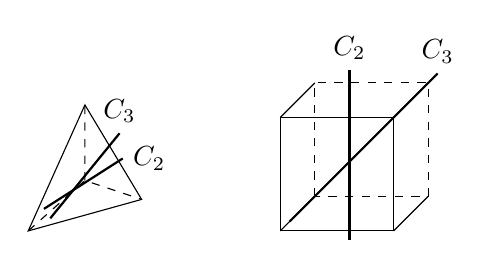
\begin{tikzpicture}[scale=.8,line width=.4pt]
\draw (0,0)--(1.8,.5)--(.9,2)--cycle; \draw[dashed] (0,0)--(.9,.8)--(1.8,.5) (.9,.8)--(.9,2);
\draw[thick] (.35,.2)--(1.45,1.55) node[above] {$C_3$}; \draw[thick] (.25,.35)--(1.5,1.15) node[right] {$C_2$};
\begin{scope}[xshift=4cm]
\draw (0,0) rectangle (1.8,1.8); \draw[dashed] (.55,.55) rectangle (2.35,2.35); \draw (0,0)--(.55,.55) (1.8,0)--(2.35,.55) (1.8,1.8)--(2.35,2.35) (0,1.8)--(.55,2.35);
\draw[thick] (.15,.15)--(2.5,2.5) node[above] {$C_3$}; \draw[thick] (1.1,-.15)--(1.1,2.55) node[above] {$C_2$};
\end{scope}
\end{tikzpicture}
\caption{}
\label{fig:93-36}
\end{figure}

The three twofold axes are mutually equivalent. The threefold axes are also equivalent, since rotations $C_2$ carry them into one another, but they are not two-sided. The 12 elements of $\boldsymbol{T}$ therefore divide into four classes: $E$, three rotations $C_2$, four rotations $C_3$, and four rotations $C_3^2$.

\medskip
\noindent IX. Group $\boldsymbol{T}_d$

This group contains every symmetry transformation of a tetrahedron. Its axes and planes arise by adding to $\boldsymbol{T}$ symmetry planes, each passing through one twofold and two threefold axes. The twofold axes thereby become fourfold rotation--reflection axes, as in $\boldsymbol{D}_{2d}$. It is convenient to draw the three rotation--reflection axes through centers of opposite cube faces, the four threefold axes along body diagonals, and the six symmetry planes

\SourcePage{445}{448}
through pairs of opposite edges. Figure~37 shows one axis and plane of each type.

Since the symmetry planes are vertical relative to the threefold axes, those axes are two-sided. All axes or planes of a given type are equivalent. The 24 elements consequently form five classes: $E$; eight rotations $C_3$ and $C_3^2$; six plane reflections; six rotation--reflection transformations $S_4$ and $S_4^3$; and three rotations $C_2=S_4^2$.

\begin{figure}[ht]
\centering
\begin{tikzpicture}[scale=.62,line width=.4pt]
\draw[dashed] (0,0) rectangle (2,2); \draw[dashed] (.7,.7) rectangle (2.7,2.7);
\draw[dashed] (0,0)--(.7,.7) (2,0)--(2.7,.7) (2,2)--(2.7,2.7) (0,2)--(.7,2.7);
\draw[pattern=vertical lines] (0,0)--(2.7,.7)--(2.7,2.7)--(0,2)--cycle;
\draw[thick] (1.35,.35)--(1.35,2.9) node[above] {$S_4$};
\draw[thick] (-.2,2.1)--(2.85,.62); \node[above left=-3pt] at (0,2.15) {$C_3$};
\node[right] at (2.72,1.9) {$\sigma$};
\begin{scope}[xshift=4.6cm,yshift=.1cm]
\draw[dashed] (0,.15)--(1.65,0)--(2.15,.95)--cycle;
\draw[dashed] (0,.15)--(.95,2.35) (1.65,0)--(.95,2.35) (2.15,.95)--(.95,2.35);
\draw[pattern=vertical lines] (.95,2.35)--(2.15,.95)--(.82,.07)--cycle;
\draw[thick] (.95,2.45)--(1.32,.05); \node[above] at (.95,2.45) {$C_3$};
\draw[thick] (1.62,1.72)--(.62,-.25); \node[below left=-3pt] at (.68,-.15) {$S_4$};
\node at (1.42,1.05) {$\sigma$};
\node at (1.1,-.55) {$T_d$};
\end{scope}
\end{tikzpicture}
\caption{}
\label{fig:93-37}
\end{figure}

\medskip
\noindent X. Group $\boldsymbol{T}_h$

This group is obtained from $\boldsymbol{T}$ by adding a center of symmetry: $\boldsymbol{T}_h=\boldsymbol{T}\times\boldsymbol{C}_i$. Three mutually perpendicular symmetry planes then appear, each passing through a pair of twofold axes, while the threefold axes become sixfold rotation--reflection axes. One such axis and one plane are shown in Fig.~38.

Its 24 elements are distributed among eight classes obtained directly from the classes of $\boldsymbol{T}$.

\medskip
\noindent XI. Group $\boldsymbol{O}$ (octahedral group)

The axial system of this group is that of a cube: three fourfold axes pass through centers of opposite faces, four threefold axes through opposite vertices, and six twofold axes through midpoints of opposite edges (Fig.~39).

\begin{figure}[ht]
\centering
\begin{tikzpicture}[scale=.62,line width=.4pt]
\draw[dashed] (0,0) rectangle (2,2); \draw[dashed] (.5,.5) rectangle (2.5,2.5);
\draw[dashed] (0,0)--(.5,.5) (2,0)--(2.5,.5) (2,2)--(2.5,2.5) (0,2)--(.5,2.5);
\draw[pattern=vertical lines] (1,0)--(1.5,.5)--(1.5,2.5)--(1,2)--cycle;
\draw[thick] (1.25,.25)--(1.25,2.85) node[above] {$C_2$};
\draw[thick] (-.2,-.2)--(2.75,2.75) node[above right=-3pt] {$S_6$};
\node at (1.3,1.9) {$\sigma$}; \node at (1.25,-.5) {$T_h$};
\end{tikzpicture}
\caption{}
\label{fig:93-38}
\end{figure}

\begin{figure}[ht]
\centering
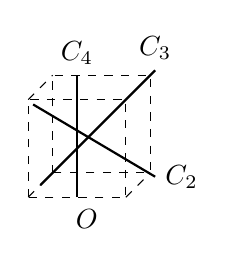
\begin{tikzpicture}[scale=.62,line width=.4pt]
\draw[dashed] (0,0) rectangle (2,2); \draw[dashed] (.5,.5) rectangle (2.5,2.5);
\draw[dashed] (0,0)--(.5,.5) (2,0)--(2.5,.5) (2,2)--(2.5,2.5) (0,2)--(.5,2.5);
\draw[thick] (1,0)--(1,2.5) node[above] {$C_4$};
\draw[thick] (.25,.25)--(2.6,2.6) node[above] {$C_3$};
\draw[thick] (.1,1.9)--(2.6,.42) node[right] {$C_2$};
\node at (1.2,-.45) {$O$};
\end{tikzpicture}
\caption{}
\label{fig:93-39}
\end{figure}

\begin{figure}[ht]
\centering
\begin{tikzpicture}[scale=.62,line width=.4pt]
\draw[dashed] (0,0) rectangle (2,2); \draw[dashed] (.5,.5) rectangle (2.5,2.5);
\draw[dashed] (0,0)--(.5,.5) (2,0)--(2.5,.5) (2,2)--(2.5,2.5) (0,2)--(.5,2.5);
\draw[pattern=vertical lines] (0,0)--(2.5,.5)--(2.5,2.5)--(0,2)--cycle;
\draw[pattern=vertical lines] (1,0)--(1.5,.5)--(1.5,2.5)--(1,2)--cycle;
\draw[thick] (1.25,.25)--(1.25,2.85) node[above] {$C_4$};
\draw[thick] (-.15,2.09)--(2.65,.41) node[right] {$C_2$};
\draw[thick] (-.15,-.15)--(2.7,2.7) node[above right=-3pt] {$S_6$};
\node at (.4,1.45) {$\sigma$}; \node at (1.28,2.2) {$\sigma$};
\node at (1.25,-.5) {$O_h$};
\end{tikzpicture}
\caption{}
\label{fig:93-40}
\end{figure}

All axes of the same order are plainly equivalent, and every axis is two-sided. The 24 elements thus divide into five classes: $E$; eight rotations $C_3$ and $C_3^2$; six rotations $C_4$ and $C_4^3$; three rotations $C_4^2$; and six rotations $C_2$.

\SourcePage{446}{449}
\medskip
\noindent XII. Group $\boldsymbol{O}_h$

This is the group of all symmetry transformations of a cube.\footnote{The groups $\boldsymbol{T}$, $\boldsymbol{T}_d$, $\boldsymbol{T}_h$, $\boldsymbol{O}$, and $\boldsymbol{O}_h$ are called \emph{cubic groups}.} It is produced by adding a center of symmetry to $\boldsymbol{O}$: $\boldsymbol{O}_h=\boldsymbol{O}\times\boldsymbol{C}_i$. The threefold axes of $\boldsymbol{O}$ thereby become sixfold rotation--reflection axes (the body diagonals of the cube). There also appear six symmetry planes through pairs of opposite edges and three planes parallel to the cube faces (Fig.~40). The group has 48 elements in ten classes, obtainable directly from those of $\boldsymbol{O}$. Five are the classes of $\boldsymbol{O}$ itself; the others are $I$; eight rotation--reflection transformations $S_6$ and $S_6^5$; six rotation--reflection transformations $C_4\sigma_h$ and $C_4^3\sigma_h$ about the fourfold axes; three reflections $\sigma_h$ in planes horizontal relative to those axes; and six reflections $\sigma_v$ in planes vertical relative to them.

\medskip
\noindent XIII, XIV. Groups $\boldsymbol{Y}$, $\boldsymbol{Y}_h$ (icosahedral groups)

Only exceptionally do these groups occur in nature as molecular symmetry groups. We therefore state only that $\boldsymbol{Y}$ is the group of 60 rotations about the symmetry axes of an icosahedron (a regular 20-faced solid with triangular faces) or a pentagonal dodecahedron (a regular 12-faced solid with pentagonal faces). There are six fivefold, ten threefold, and fifteen twofold axes. Adding a center of symmetry gives $\boldsymbol{Y}_h=\boldsymbol{Y}\times\boldsymbol{C}_i$, the full symmetry group of these polyhedra.

This exhausts the possible types of point groups with finitely many elements. In addition, the continuous point groups, which have infinitely many elements, must be considered; this will be done in \S~98.
